\section{Generalization through the Lens of Selective Underfitting} \label{sec:generalization}
We now characterize our \ours using the \emph{supervision region} defined in Section~\ref{sec:training-region}.
\begin{equation*}
    \rvs_\rvtheta (\rvz_t, t)=
    \begin{cases}
    \xxgreen{\approx \rvs_\star (\rvz_t, t)} & \text{(\coloredhl{xblue}{$\rvz_t \in \gT_t (\delta)$}, \emph{Supervision}) \quad$\to$ underfitting \ding{55}} \\
    \xsienna{\not\approx \rvs_\star (\rvz_t, t)} & \text{(\coloredhl{xred}{$\rvz_t \notin \gT_t (\delta)$}, \emph{Extrapolation}) \,$\to$ underfitting \ding{51}}
    \end{cases}
\end{equation*}
During training, supervision occurs only within a set of narrow shells $\xblue{\mathcal{T}_t(\delta)}$, where the empirical score $\xxgreen{\rvs_\star}$ reduces to a trivial form (\Cref{sec:training-region}). 
We claim that underfitting does \emph{not} occur in this region--the model learns toward the empirical score function. At inference time, a \xred{sampling trajectory} leaves these shells after just a few denoising steps (Section~\ref{sec:inference-extrapolation}), and in this extrapolation region, we claim the underfitting \emph{does} occur.
%
In the following \Cref{sec:selective}, we demonstrate this \emph{selective underfitting} by examining the model’s behavior across these two regions.

\subsection{Selective Underfitting} \label{sec:selective}

\begin{minipage}{0.645\textwidth}
\begin{experiment}[Supervision vs.\ Extrapolation]
\label{exp:contrastive-scaling}
We quantify ``underfitting'' as the deviation of the learned score from the empirical score, i.e., $\| \rvs_\rvtheta - \rvs_\star\|^2$. Specifically, we measure this quantity separately within the supervision and extrapolation regions, using pretrained models across various scales: SiT-\{S, B, L, XL\}. Our experiments are conducted on ImageNet, where the empirical score is computable, facilitating this analysis. \Cref{fig:contrastive-scaling} reveals that as model capacity increases (left to right), $\rvs_\theta$ approaches $\rvs_\star$ in the supervision region (\coloreddashul{xblue}{blue line}), indicating that underfitting does not occur there.
Conversely, in the extrapolation region, larger models increasingly deviate from $\rvs_\star$ (\coloreddashul{xred}{red line}), indicating that underfitting occurs. This contrast provides clear evidence for selective underfitting.
\end{experiment}
\end{minipage}
\hfill
\begin{minipage}{0.34\textwidth}
\begin{figure}[H]
    \centering
    \vskip -\baselineskip
    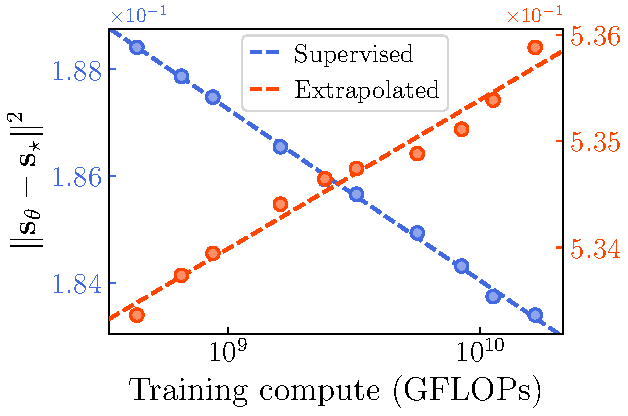
\includegraphics[width=\textwidth,trim={0.2cm 0 0.2cm 0}]{figures/generalization/contrastive_scaling}
    \vskip -0.75\baselineskip
    \caption{\textbf{Quantitative verification of selective underfitting.} $\|\rvs_\theta - \rvs_\star\|^2$ exhibits contrastive scaling behavior in \coloreddashul{xblue}{supervision region} vs.\ \coloreddashul{xred}{extrapolation region}.}
    \label{fig:contrastive-scaling}
\end{figure}
\end{minipage}

\Cref{exp:contrastive-scaling} quantitatively demonstrates that the learned score closely matches the empirical score in the supervision region. But how small is this difference in absolute terms? Below, \Cref{exp:memorization-training} shows it is small enough for the model to \emph{reproduce} training samples.

\begin{experiment}[Memorization in Supervision Region]
\label{exp:memorization-training} We take a noisy image $\xblue{\rvz_t} = \alpha_t \rvx^{(i)} + \sigma_t \rveps \sim \xblue{\hat{p}_t}$ (with $\rvx^{(i)} \in \mathcal{D}$) and use a pretrained SiT-XL model to iteratively denoise from timestep $t$ to $0$. Figure~\ref{fig:phase-transition} shows that for $t < 0.8$, sampling consistently regresses to the original image $\rvx^{(i)}$. This indicates that the model has (almost perfectly) learned the empirical score in the supervision region, thereby \xolive{\emph{memorizing}} the training image. Notably, previously observed phase transitions~\citep{georgiev2023journey,li2024critical} can be interpreted as manifestations of selective underfitting.
\end{experiment}

\newenvironment{tmpfigure}
  {\venueifelse{\begin{figure}[H]}{\begin{figure}[H]}}
  {\end{figure}}


\begin{tmpfigure}
    \centering
    \venueifelse{\vskip -0.75\baselineskip}{\vskip -0.25\baselineskip}
    \vskip -0.75\baselineskip
    \begin{subfigure}[t]{0.7\textwidth}
        \centering
        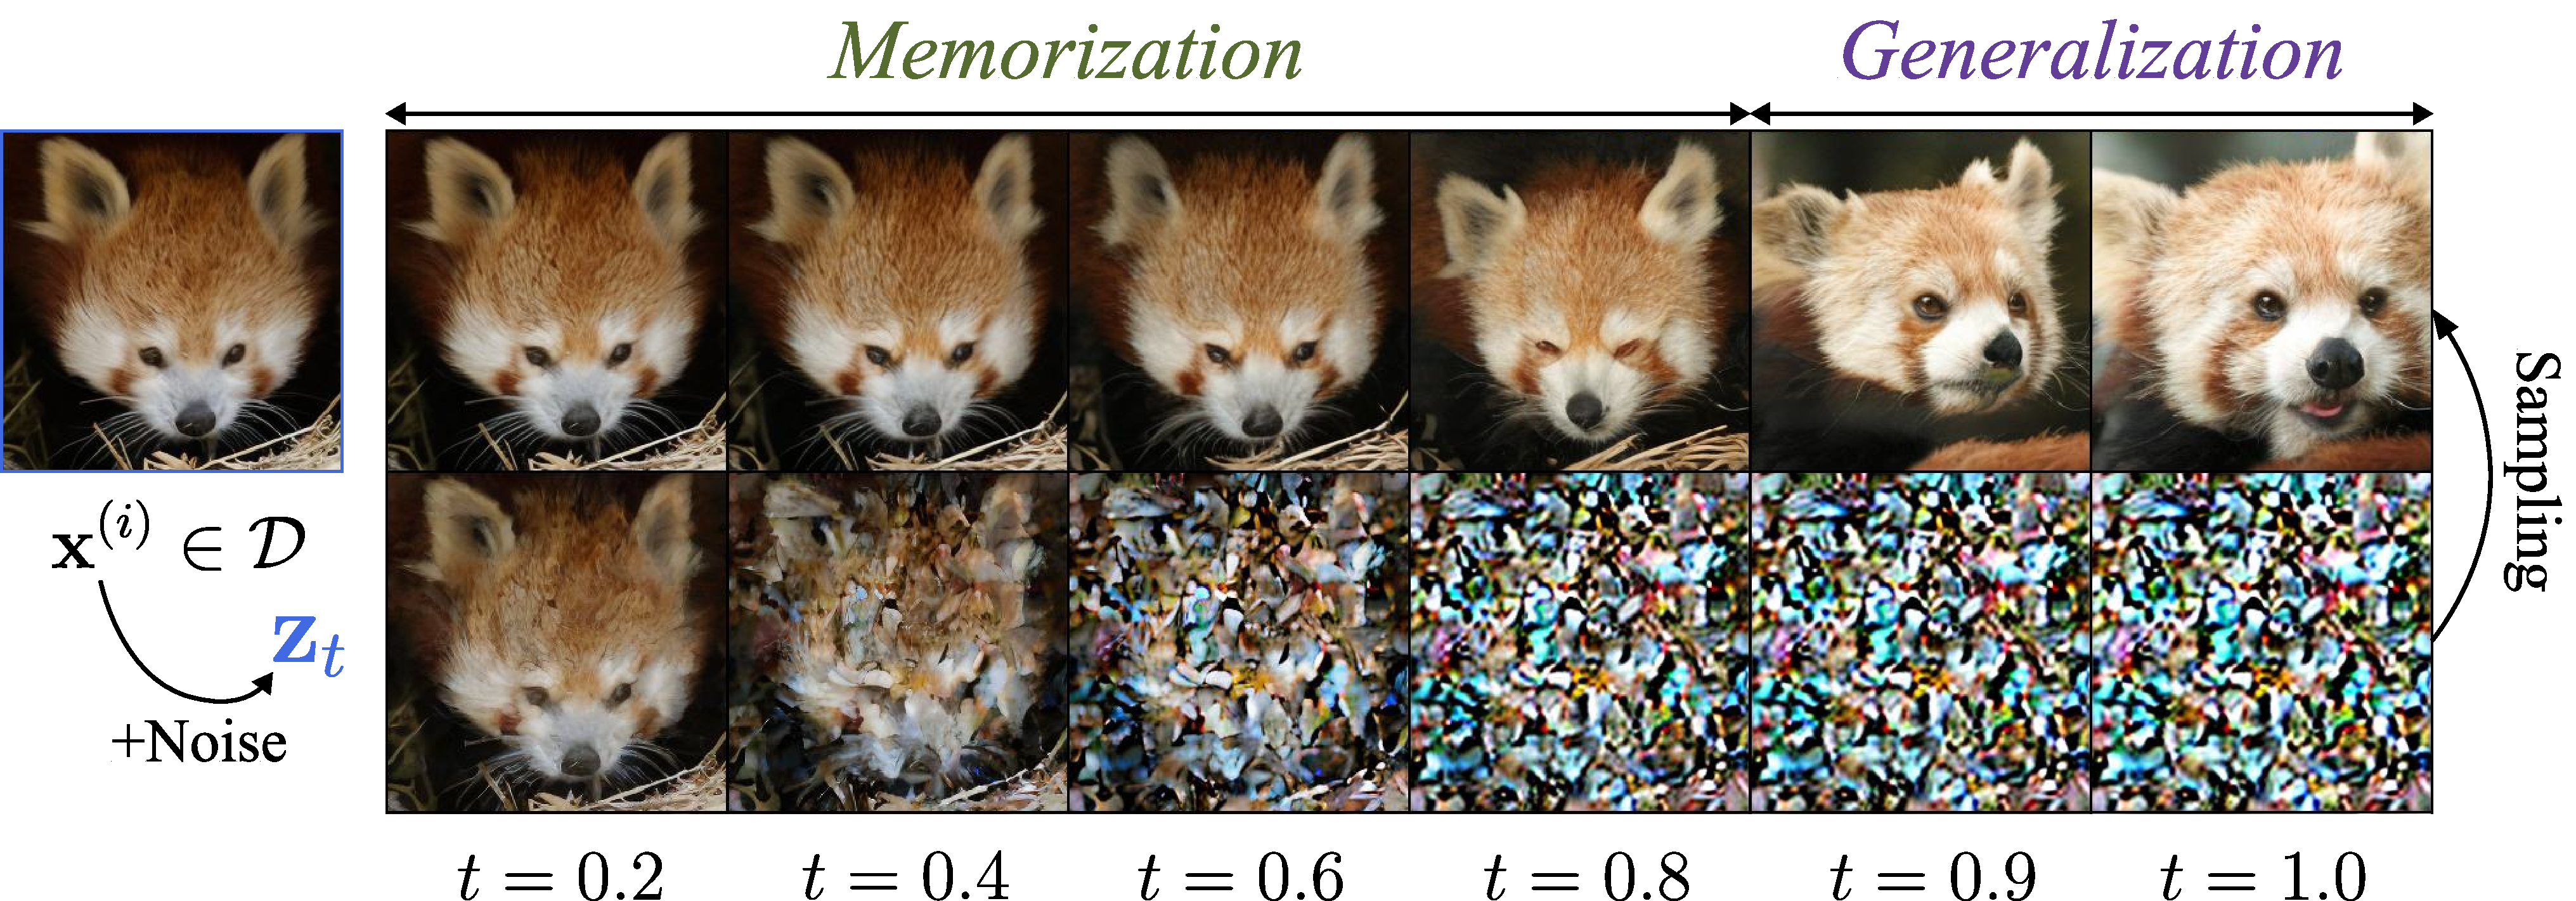
\includegraphics[width=\textwidth]{figures/generalization/phase_transition_example}
    \end{subfigure}
    \hfill
    \begin{subfigure}[t]{0.29\textwidth}
        \centering
        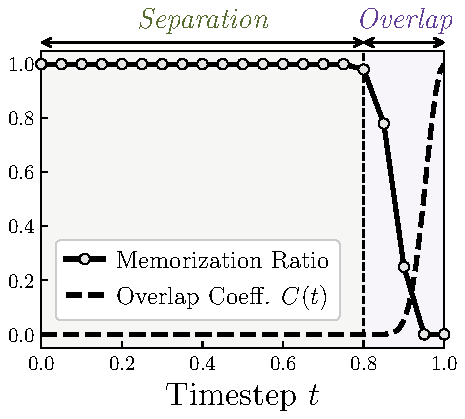
\includegraphics[width=\textwidth,trim=0 0.55cm 0 0]{figures/generalization/phase_transition_plot}
    \end{subfigure}
        \caption{\textbf{Qualitative example of selective underfitting.} \emph{Left}: Sampling ($t \to 0$) from a noisy image $\xblue{\rvz_t}$ in the supervision region maps back to the original training image $\rvx^{(i)}$ for most time steps ($t < 0.8$). \emph{Right}: The overlap coefficient $C(t)$ and memorization ratio. The \coloredul{black}{memorization ratio} exhibits the same trend quantitatively.}
    \label{fig:phase-transition}
    \venueifelse{\vskip -1.5\baselineskip}{\vskip -0.5\baselineskip}
\end{tmpfigure}

\textbf{Selective Underfitting Persists in Gaussian Distribution.} A natural follow-up question is whether this persists even when the ground-truth distribution is simple. Here, the ground truth distribution conceptually denotes the distribution from which the training data are drawn. (For images, this notion is ill-defined and outside our scope). We consider a simple synthetic setup where the ground truth distribution is Gaussian, whose score is linear: in principle, a neural network could fit this linear function globally, i.e., globally underfit the empirical score, rather than 
adopting a more complex selective underfitting.  Nevertheless, selective underfitting is still observed, suggesting the phenomenon persists even for simple distributions, warranting theoretical investigation of \emph{selective underfitting} (see the result in \Cref{app:selective-gaussian}).

\subsection{Freedom of Extrapolation: A Mechanism Behind Generalization} \label{sec:freedom}
We now show how \ours offers a novel perspective on diffusion model generalization--one that prior perspectives could not support. The diffusion model generalization refers to a model's ability to generate unseen (creative) data samples. As noted in the introduction, if a model perfectly learns the empirical score function, it would simply regenerate the training set; this is puzzling, since the DSM loss (\Cref{eq:dsm})'s unique minimizer is the empirical score.

The prevailing account, following \common, posits that training-time bias causes the learned score to underfit globally across the data space, leading to a favorable score function. In contrast, we propose that the learned score results from \emph{selective underfitting}--distinct behavior in the supervision versus extrapolation regions. We now show that this distinction is key to generalization by claiming:
\begin{claim} \label{claim:freedom}
Diffusion models fail to generalize when the supervision region is broadened.
\end{claim}
The intuition is that the learned score function is sensitive to the size of the supervision region. Consider two diffusion models trained to minimize $\mathbb{E}_{\rvz_t \sim \xblue{q_t}} \,\|\,\rvs_\rvtheta(\rvz_t,t)-\xxgreen{\rvs_\star(\rvz_t,t)}\,\|^2$ under different training distributions $\xblue{q_t}$ but with the same $\xxgreen{\rvs_\star}$. Despite sharing the same empirical score, they can learn markedly different score functions—and hence exhibit different generalization. We refer to this intuition as \emph{Freedom of Extrapolation}: the more \emph{freedom} the model has to extrapolate beyond the supervision region, the better its generalization tends to be.

In standard DSM training (\Cref{fig:foe-generalization}), the network is supervised within a restricted supervision region (\coloredul{xblue}{blue}) while retaining \emph{freedom to extrapolate} (underfit) elsewhere (\coloredul{xsienna}{brown}). Conversely, in \Cref{fig:foe-memorization}, enlarging the supervision region (\coloredul{xblue}{blue}) shrinks the space available for extrapolation, yielding \emph{limited freedom to extrapolate} (\coloredul{xsienna}{brown}). This behavior cannot be explained by \common, which lacks a notion of a supervision region. We verify this claim with a controlled experiment below.

\newcommand{\trainr}{\xblue{\train_\text{region}}}
\newcommand{\trainrp}{\train_\text{region}}
\newcommand{\trainrabs}{\xblue{|\train_\text{region}|}}
\newcommand{\trainrabsp}{|\train_\text{region}|}
\newcommand{\trains}{\xxgreen{\train_\text{score}}}
\newcommand{\trainsp}{\train_\text{score}}
\newcommand{\trainsabs}{\xxgreen{|\train_\text{score}|}}
\newcommand{\trainsabsp}{|\train_\text{score}|}
\newcommand{\trainabs}{|\train|}

\begin{figure}[b]
    \vskip -1.5\baselineskip
    \centering
    \begin{subfigure}[t]{0.32\textwidth}
        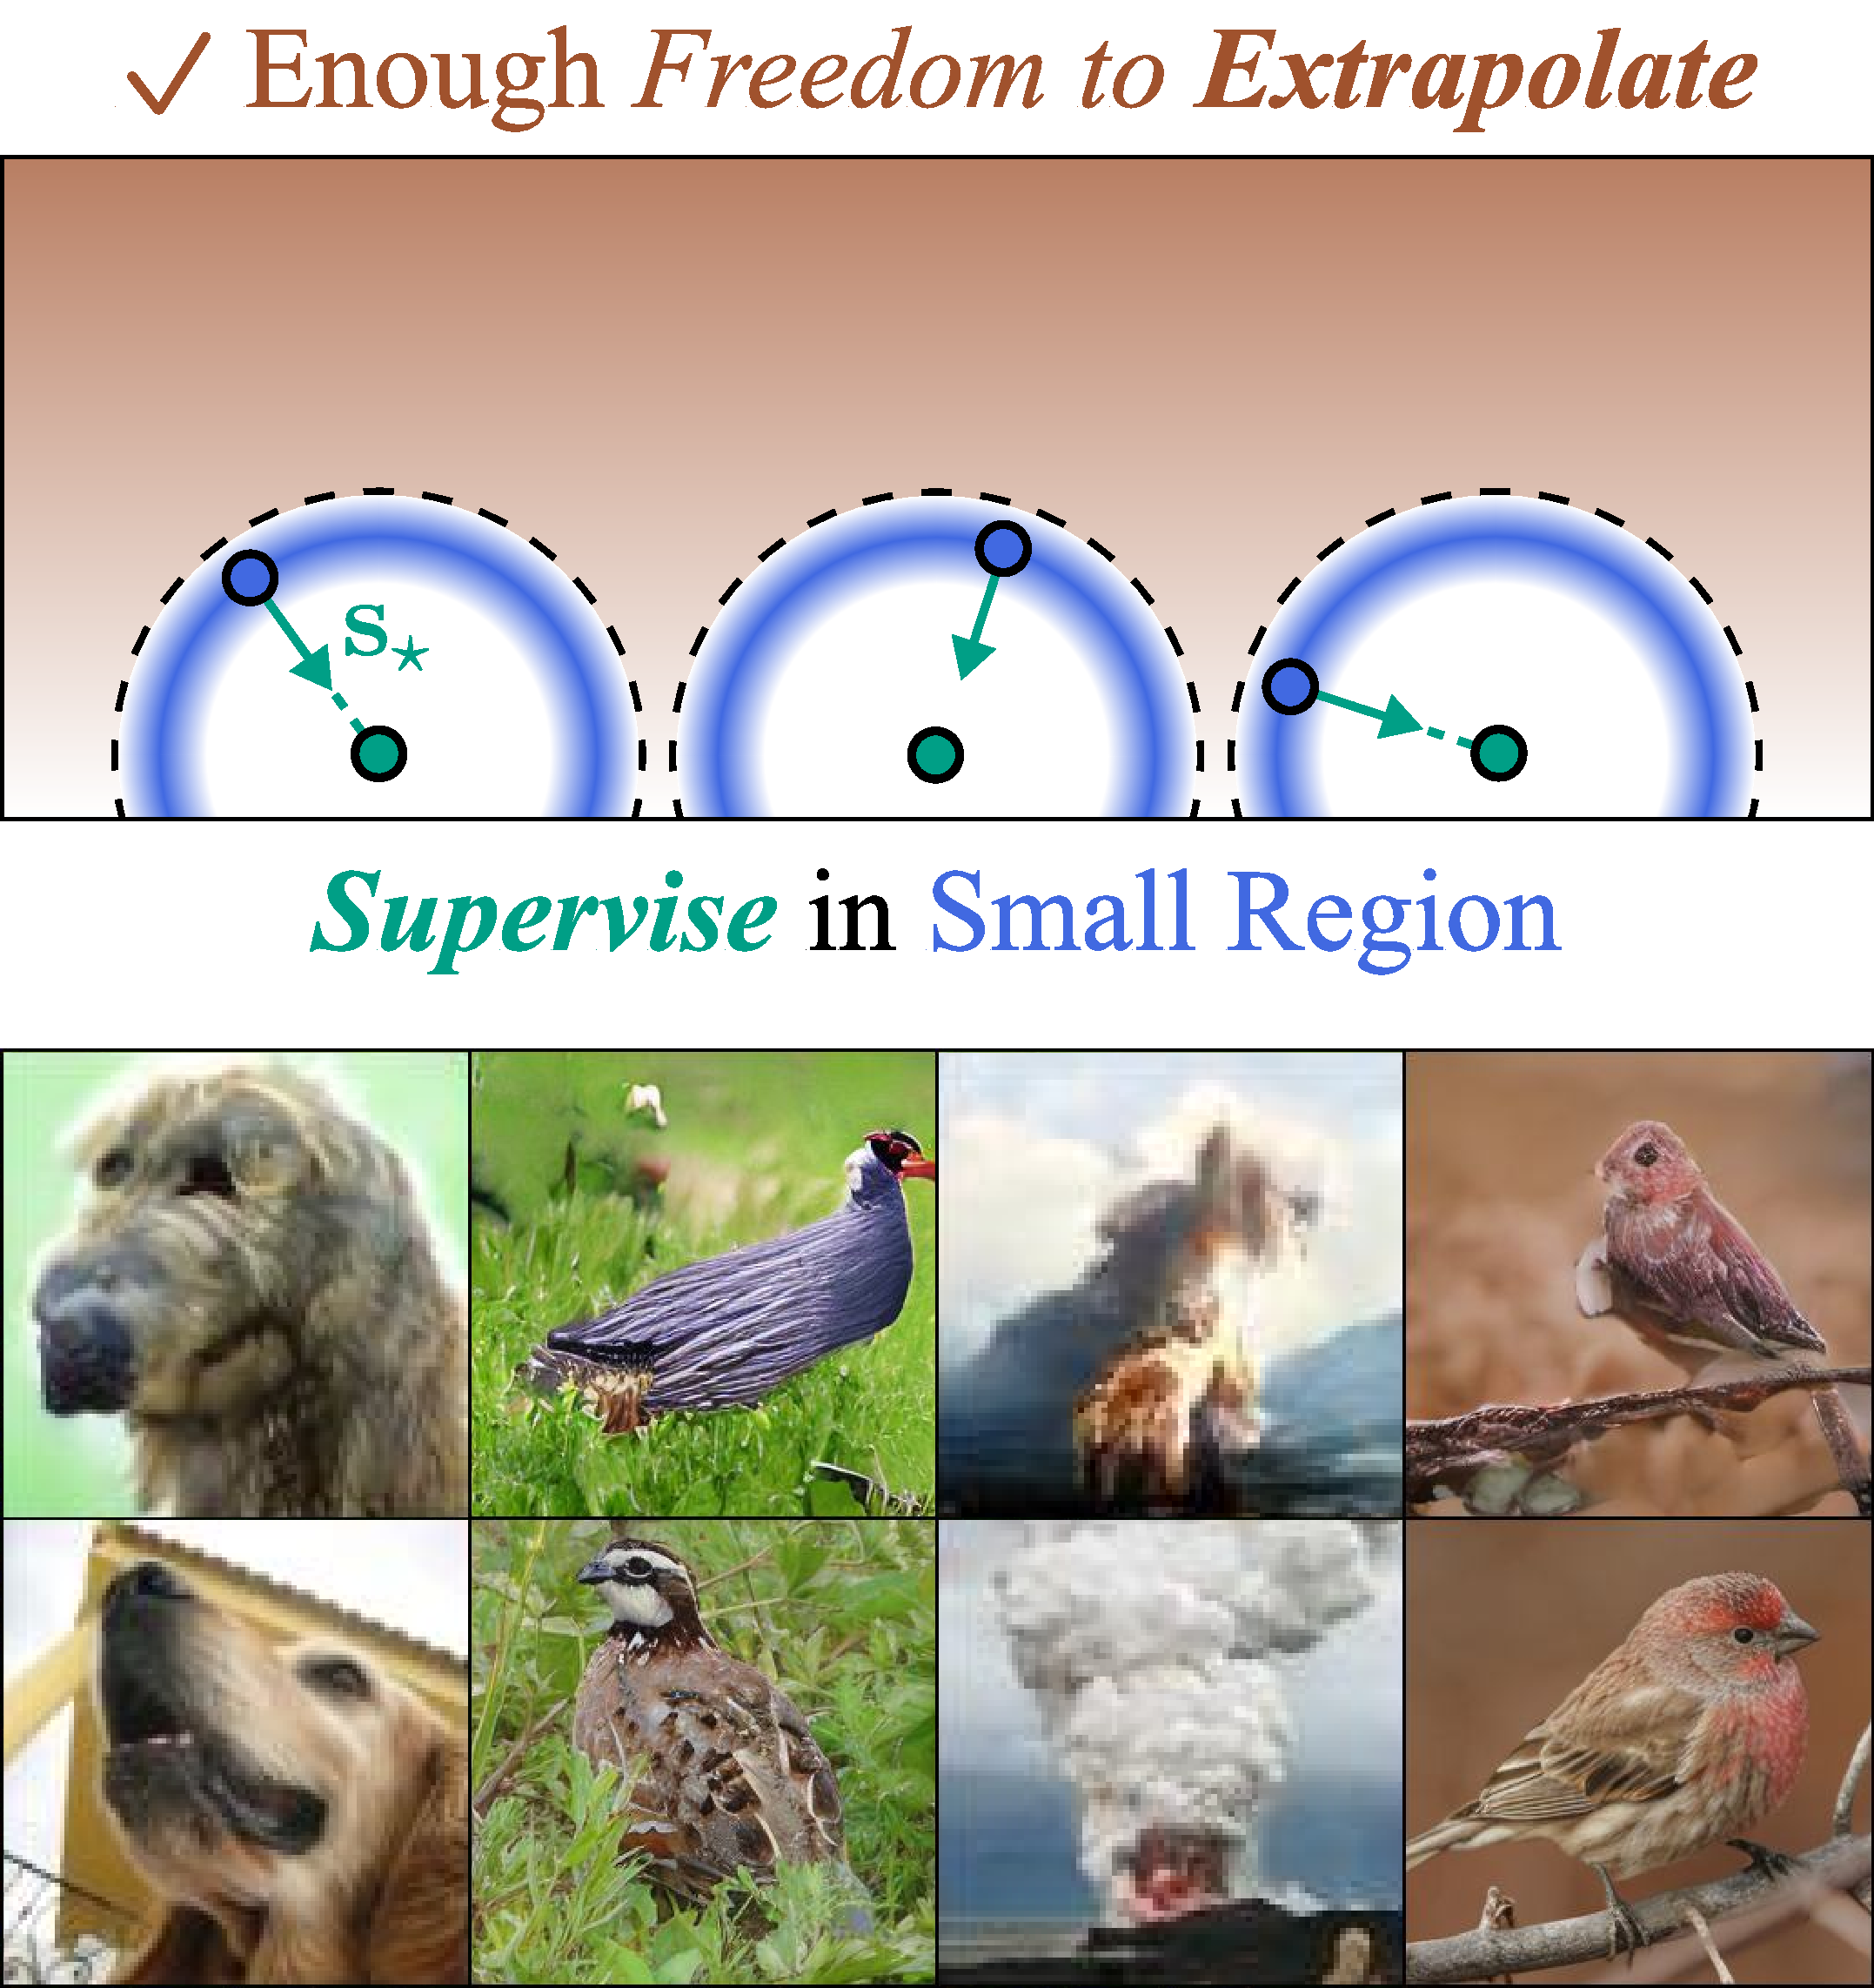
\includegraphics[height=0.99\textwidth]{figures/generalization/foe_generalization}
        \caption{\textbf{\xxpurple{Generalization.}} \xblue{Small supervision region} ($\trainrabsp = \trainsabsp$) \xsienna{ensures \emph{freedom to extrapolate}}.}
        \label{fig:foe-generalization}
    \end{subfigure}
    \hfill
    \begin{subfigure}[t]{0.32\textwidth}
        \centering
        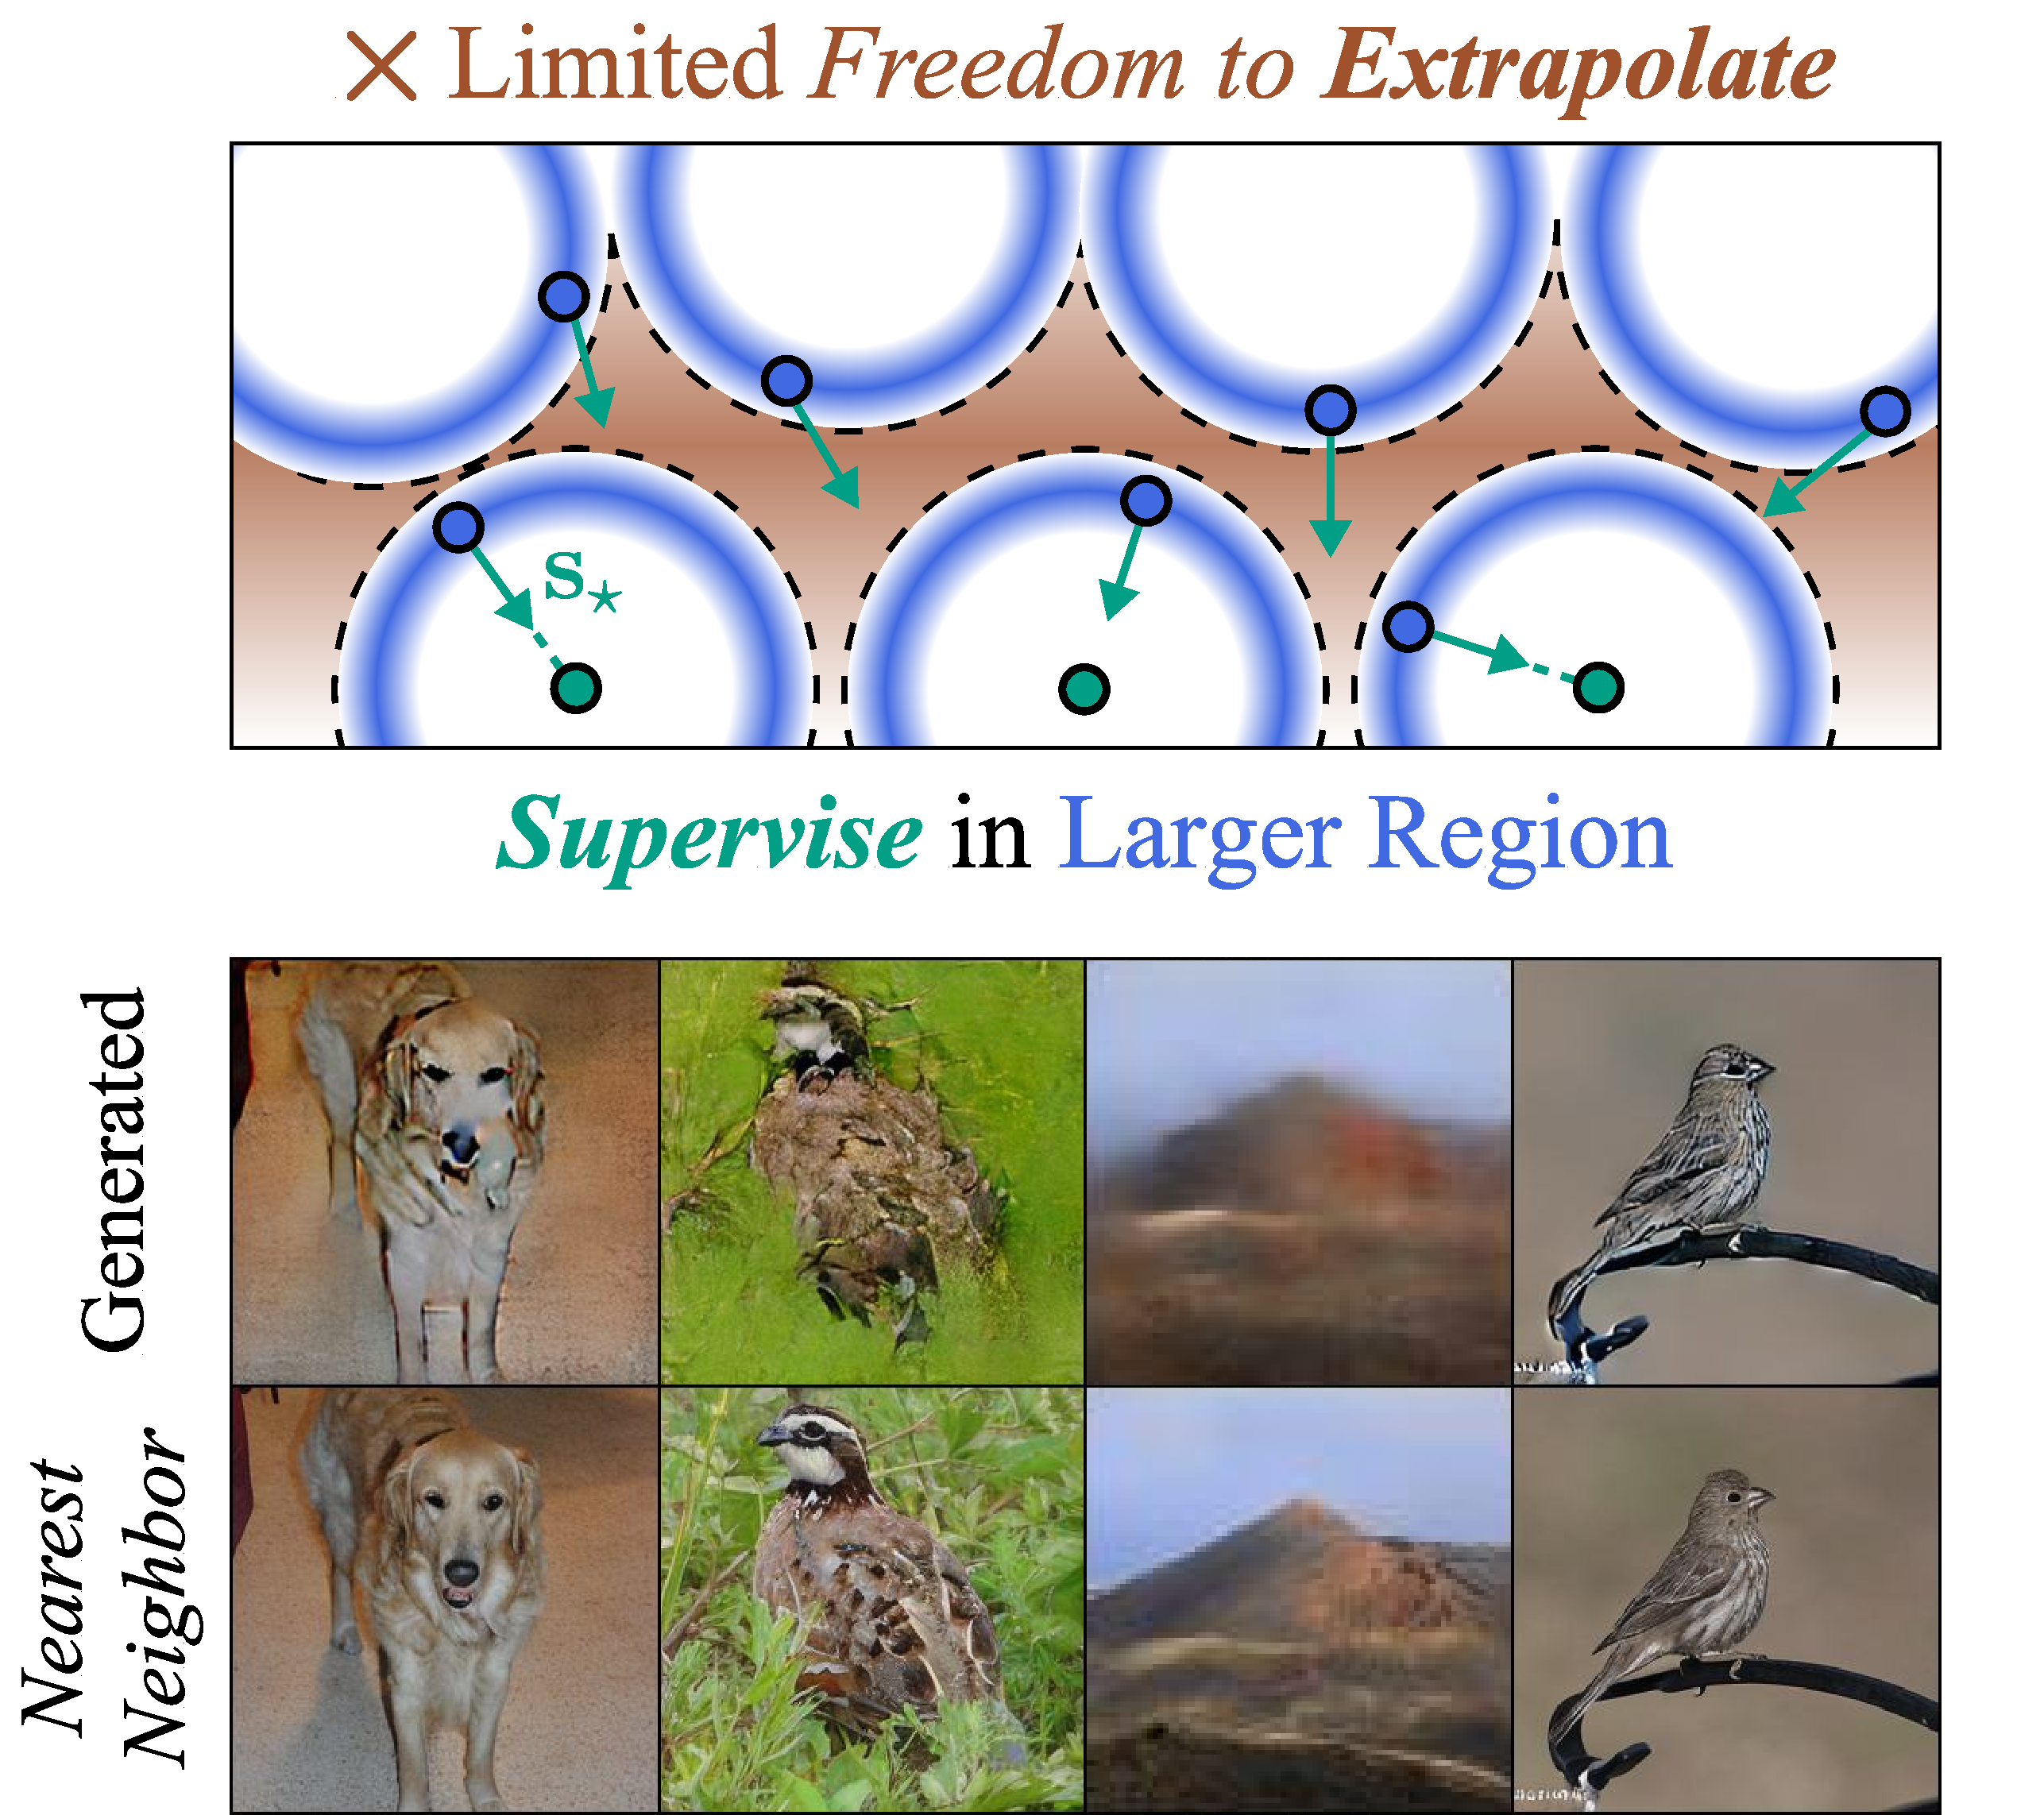
\includegraphics[height=0.99\textwidth,trim=4.1cm 0 0 0]{figures/generalization/foe_memorization}
        \caption{\textbf{\xolive{Memorization.}} \xblue{Larger supervision region} ($\trainrabsp \gg \trainsabsp$) \xsienna{limits \emph{freedom to extrapolate}}.}
        \label{fig:foe-memorization}
    \end{subfigure}
    \hfill
    \begin{subfigure}[t]{0.33\textwidth}
        \centering
        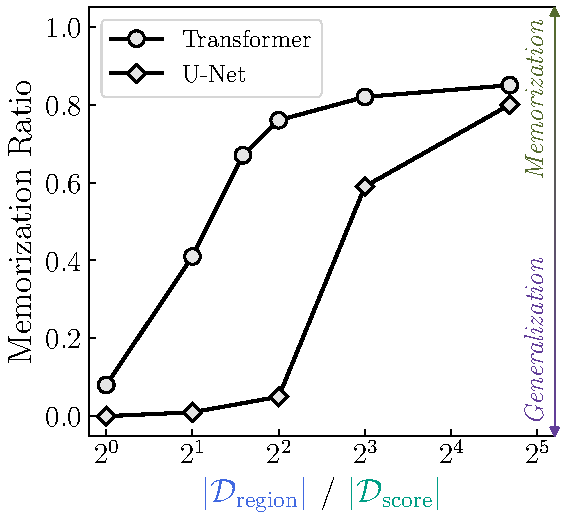
\includegraphics[height=0.85\textwidth,trim=0.2cm 0.15cm 0.3cm 0.45cm]{figures/generalization/foe_plot}
        \caption{\textbf{Quantitatively,} enlarging the supervision region $\trainr$ increases the ratio of \xolive{\emph{memorized}} samples.}
        \label{fig:foe-plot}
    \end{subfigure}
    \vskip -0.4\baselineskip
    \caption{\textbf{Experimental verification of \xsienna{\emph{freedom of extrapolation}} on ImageNet.} Deliberately limiting the \emph{freedom to extrapolate} transforms the diffusion model from \xxpurple{\emph{generalization}} to \xolive{\emph{memorization}}.}
    \label{fig:foe}
\end{figure}

\begin{experiment}[Experimental Verification] \label{exp:foe}
We train a series of models that all learn the same empirical score function, but over varying size of supervision regions--specifically, by changing the (effective) support of $\xblue{\hat{p}_t}$ while keeping $\xxgreen{s_\star}$ fixed in the objective $\E_{\rvz_t \sim \xblue{\hat{p}_t}} \left\| \rvs_\rvtheta (\rvz_t, t) - \xxgreen{\rvs_\star (\rvz_t, t)} \right\|^2$. To do this, we select two (random) subsets from the ImageNet training set $\train$: the \emph{score subset} $\trains$ and the \emph{region subset} $\trainr$, with $\trainsp \subseteq \trainrp \subseteq \train$. In the training objective, two subsets play distinct roles: $\trains$ defines the empirical score $\xxgreen{s_\star}$, while $\trainr$ determines the supervision region $\xblue{\hat{p}_t}$. Concretely, we sample $\rvz_t \sim \hat{p}_t$ by adding noise to points from $\trainrp$, and minimize $\mathbb{E}_{\rvz_t \sim \hat{p}_t} \left\| \rvs_\rvtheta (\rvz_t, t)-\rvs_\star (\rvz_t, t)\right\|^2$, where $s_\star$ is computed with respect to $\trainsp$. Consequently, varying only 
$|\trainrp|$ lets us cleanly assess how the supervision-region size affects generalization.

We present the results in \Cref{fig:foe}, fixing $\trainsabsp$ and varying $\trainrabsp$ from $\trainsabsp$ to $\trainabs$. Regardless of architecture, when $\trainrabsp = \trainsabsp$ (\emph{with freedom of extrapolation}), the model \xxpurple{\emph{generalizes}}; when $\trainrabsp \gg \trainsabsp$ (\emph{without freedom of extrapolation}), the model \xolive{\emph{memorizes}}, verifying \hyperref[claim:freedom]{\textbf{C3}}. 
\end{experiment}
\textbf{Connection to Benign Overfitting.} 
Benign overfitting \citep{bartlett2020benign,zou2021benign,frei2023benign} in classical supervised learning posits that implicit training biases (e.g., from the optimizer or regularization) guide the learner toward a “favorable” interpolating solution—one that attains zero training loss that generalizes to test data. Our selective underfitting in diffusion models is analogous: the learned score \emph{overfits} the empirical score in the supervision region, while there remain infinitely many extrapolations yielding nearly the same training loss--and \emph{freedom of extrapolation} allows the model to select a favorable score function that generalizes. A difference is that the DSM loss is averaged over the entire data space, so the training loss cannot be zero even if a model fits the empirical score in the supervision region. This analogy opens a path to translating insights from classical supervised learning into a theory of generalization for diffusion models.

\textbf{Discussion.} Our claim in \hyperref[claim:freedom]{\textbf{C3}} posits that the narrow supervision used in DSM grants diffusion models the \emph{freedom to extrapolate} beyond the supervision region, and that this freedom is central to generalization. Our architecture-agnostic experiments show that this effect persists regardless of inductive bias. \xxpurple{\textbf{This behavior cannot be explained by previous \common~\citep{kamb2024analytic,niedoba2024towards}, which focus on \emph{how} inductive bias shapes underfitting of the empirical score.}} \xsienna{\textbf{Our \ours adds a complementary dimension: to fully understand diffusion model generalization, one must consider \emph{where} the model underfits, not only \emph{how}}}.